\documentclass{article}

\usepackage{amsmath,amssymb,bm}
\usepackage{graphicx}
\usepackage{natbib}
\usepackage[latin1]{inputenc}
%\usepackage[english,french]{babel}
%\usepackage{lineno}
\usepackage{tikz}
\setlength{\doublerulesep}{\arrayrulewidth}
\usepackage{setspace}

%%%% Comment these two lines to get journal format %%%
%\renewcommand{\baselinestretch}{1.8} % the double line spacing
%\usepackage{endfloat}
%%%%

\usepackage{verbatim}
%\usepackage[x11names, rgb]{xcolor}
%\usepackage{tikz}

\newcommand{\ie}{i.e.\ }
\newcommand{\eg}{e.g.\ }

%\linenumbers
\textwidth=17cm
\marginparwidth=0cm
\hoffset=-2cm

\begin{document}
\begin{center}
\Large Transmitter experiments\\ \normalsize
Martin W.\ Pedersen, Kevin Weng, Chase\\
Compiled: \today  
\end{center}

\textbf{Abstract}\\
Questions: 
\begin{enumerate}
\item How do cases affect signal strength?
\item How does the number of tags in the water affect the proportion of received pings?
\item How accurate is Vemco's specification of ping rate and ping delay?
\end{enumerate}

 
\section{Results}
\label{sec:results}

\subsection{Experiment 1 - effect of cases}

See Figures~\ref{fig:ex1t1}-~\ref{fig:ex1t3}.

\begin{figure}
  \begin{center}
    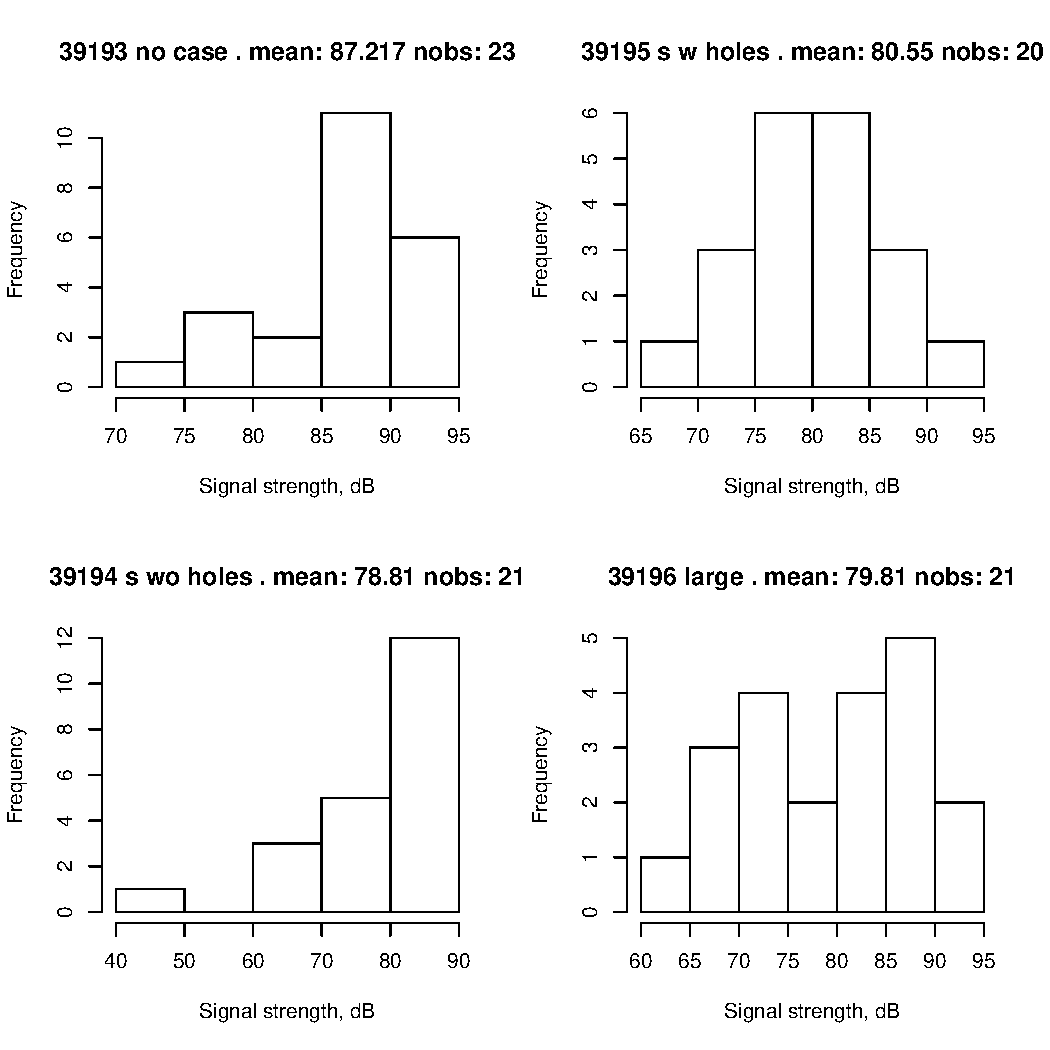
\includegraphics[trim=0cm 0cm 0cm 0cm,clip,angle=0,width=1\textwidth]{experiment1/casesTrial1.pdf}
  \end{center}
  \caption{Trial 1}
\label{fig:ex1t1}
\end{figure}

\begin{figure}
  \begin{center}
    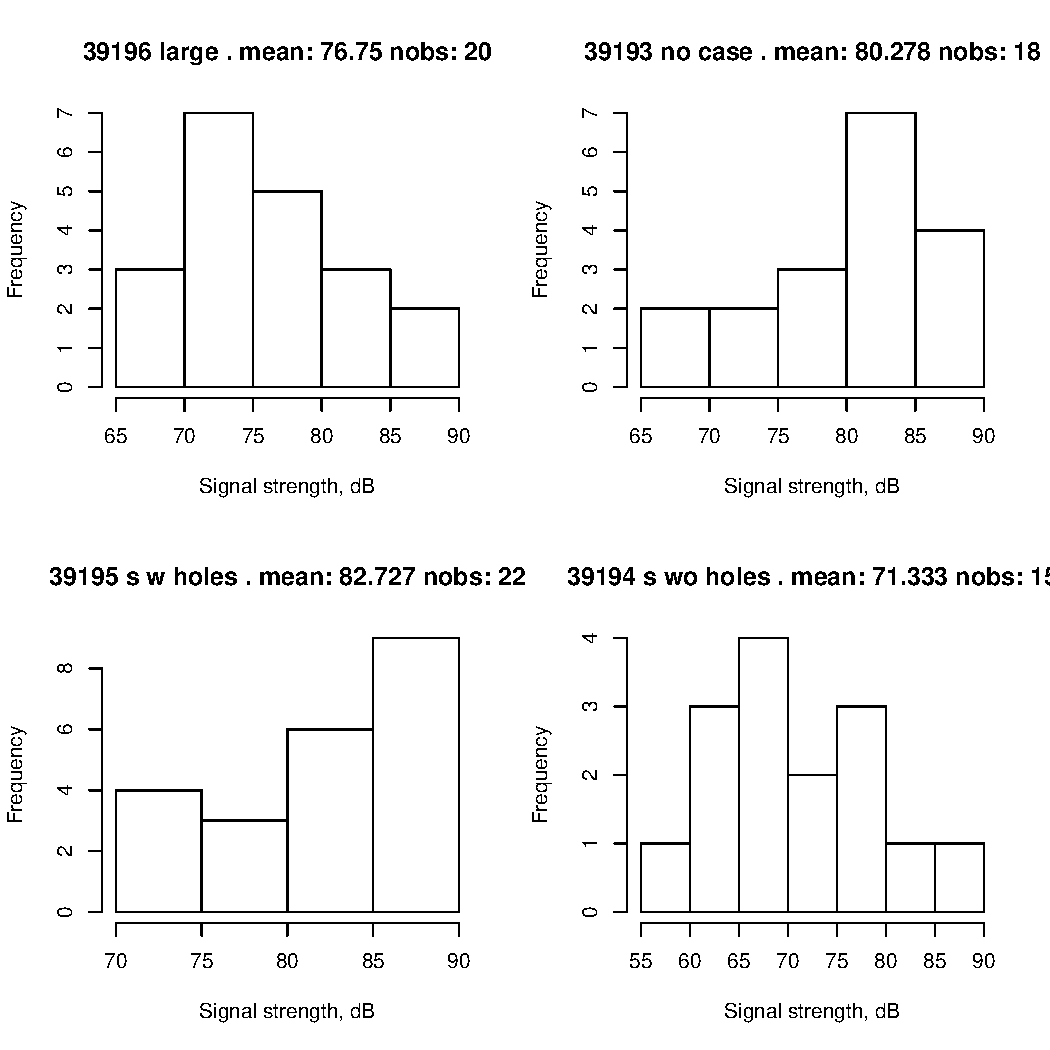
\includegraphics[trim=0cm 0cm 0cm 0cm,clip,angle=0,width=1\textwidth]{experiment1/casesTrial2.pdf}
  \end{center}
  \caption{Trial 2}
\label{fig:ex1t2}
\end{figure}

\begin{figure}
  \begin{center}
    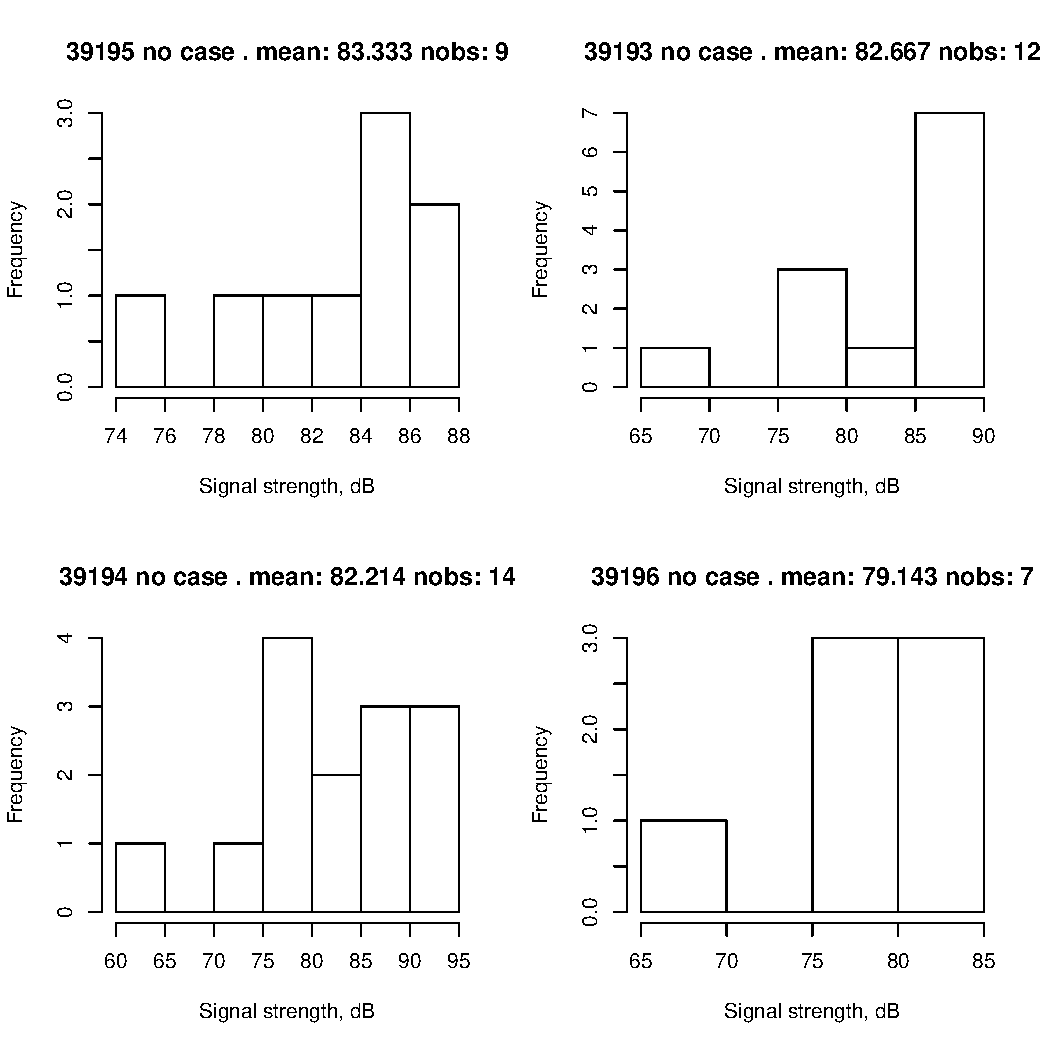
\includegraphics[trim=0cm 0cm 0cm 0cm,clip,angle=0,width=1\textwidth]{experiment1/casesTrial3.pdf}
  \end{center}
  \caption{Trial 3}
\label{fig:ex1t3}
\end{figure}

\subsection{Experiment 2 - collisions}

See Figure~\ref{fig:ex2}.

\begin{figure}
  \begin{center}
    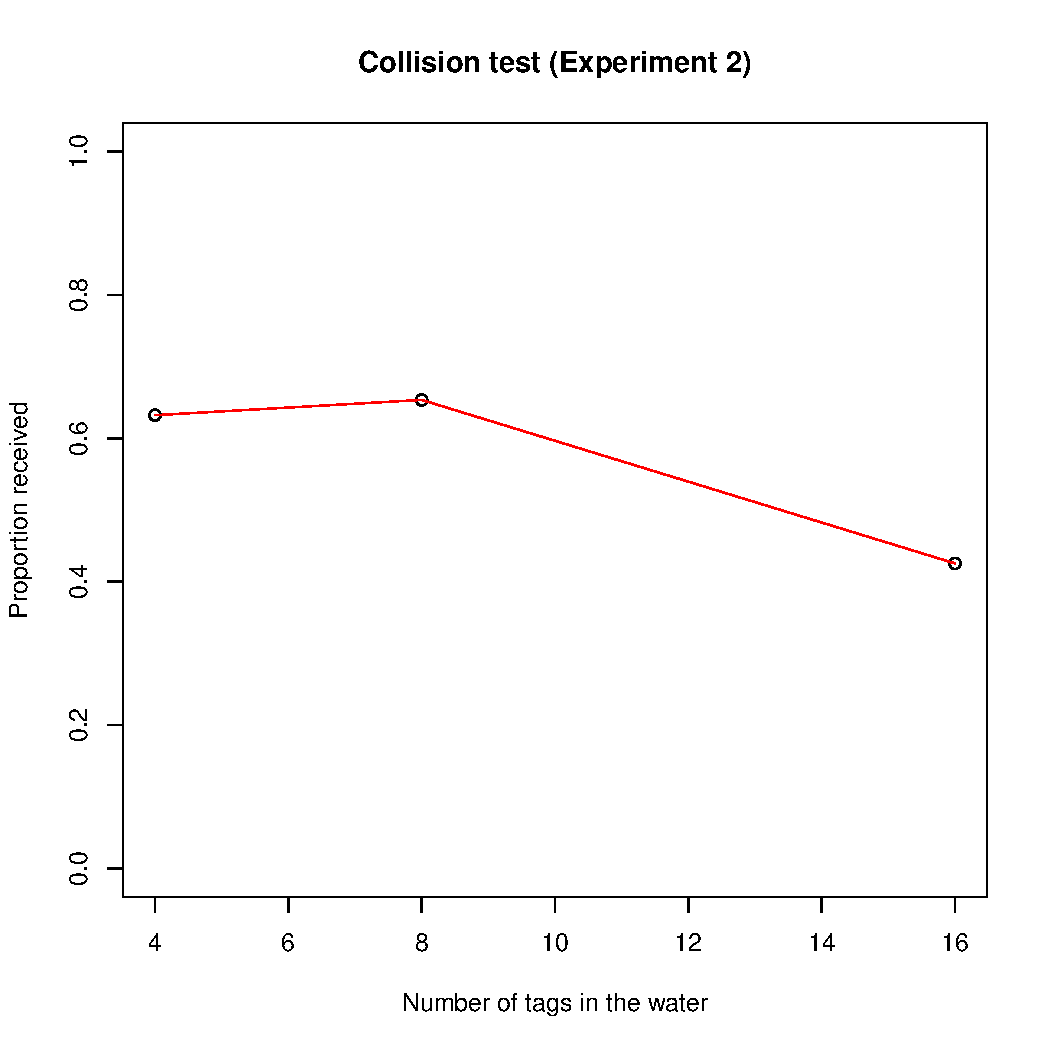
\includegraphics[trim=0cm 0cm 0cm 0cm,clip,angle=0,width=1\textwidth]{experiment2/collresult.pdf}
  \end{center}
  \caption{Collision experiment.}
\label{fig:ex2}
\end{figure}

\subsection{Experiment 3 - ping rate}

See Figure~\ref{fig:ex3}.

\begin{figure}
  \begin{center}
    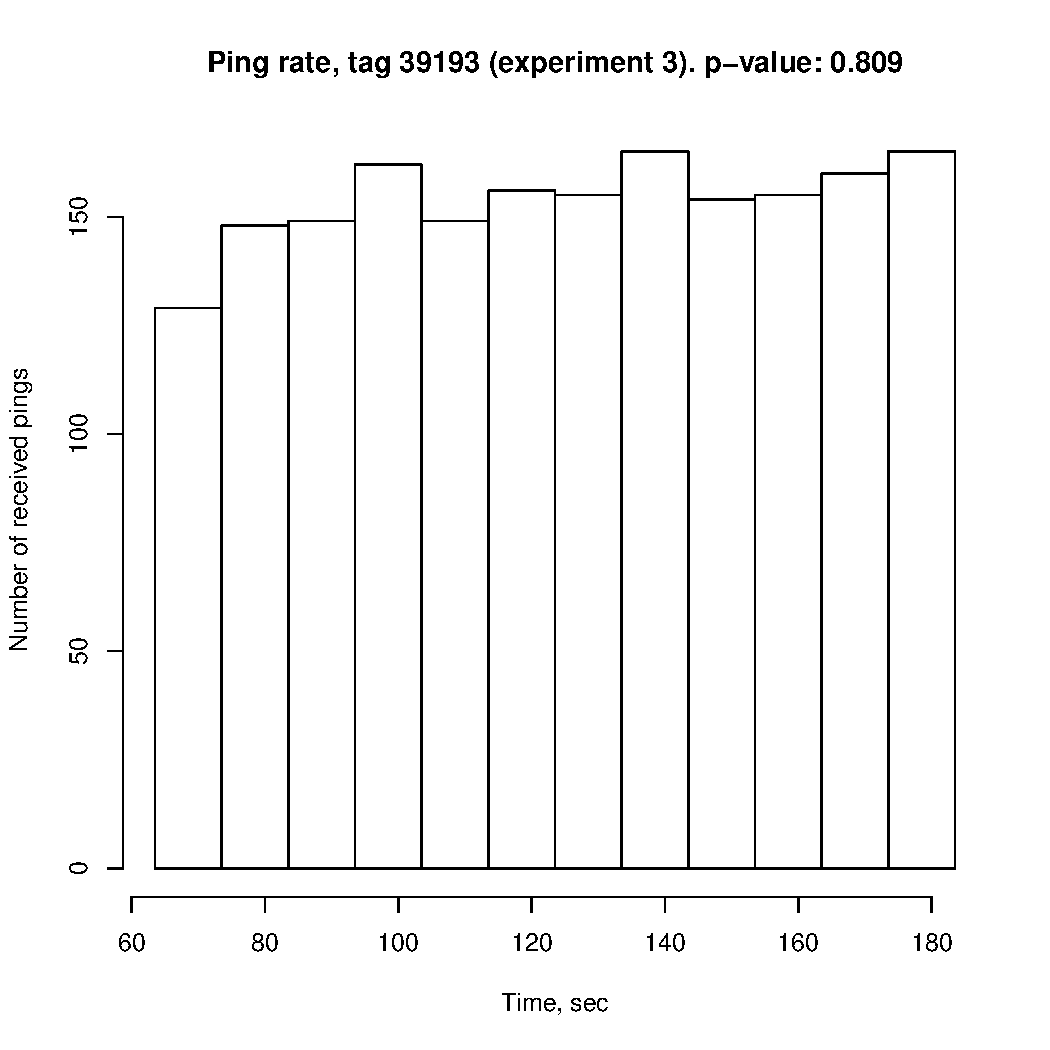
\includegraphics[trim=0cm 0cm 0cm 0cm,clip,angle=0,width=1\textwidth]{experiment3/pingrate.pdf}
  \end{center}
  \caption{Ping rate.}
\label{fig:ex3}
\end{figure}

%\bibliographystyle{elsarticle-harv}
\bibliography{/home/mwp/work/refs/refs}

\end{document}
